\documentclass[8pt]{beamer}

\usefonttheme{serif}
\usetheme{CambridgeUS}

\usepackage[utf8]{inputenc} %utf8
%\usepackage[italian]{babel}
\usepackage[T1]{fontenc}
\author{Roberto Biondo}
\institute{\small Dipartimento di Informatica\\Università di Pisa}
\title{\textbf{On Adhesivity of EGGs}}
\usepackage{datetime}
\newdate{date}{29}{11}{2024}
\date{\displaydate{date}}


\usepackage{wrapfig}
\usepackage[T1]{fontenc} % Font encoding, T1 = it
%\usepackage[size=a4]{breamerposter}
\usepackage[utf8]{inputenc} % Input encoding - per caratteri particolari
%\usepackage[english]{babel} % Lingua principale inglese
\usepackage{graphicx} % Per includere immagini esterne
%\usepackage[tickmarkheight=.5em,textwidth=\marginparwidth,textsize=small]{todonotes}
%\usepackage[a4paper,top=3cm,bottom=3cm,left=3cm,right=3cm]{geometry} %impaginazione e margini documento -- DA POROBLEMI!!!
%\usepackage[fontsize=12pt]{scrextend} %dimensione font

%\usepackage{titlesec} %indice

\usepackage{csquotes}

%\usepackage[all,cmtip]{xy}

\usepackage{amssymb,amsthm, amsmath, mathrsfs, dsfont} %simboli matematici
\usepackage{subcaption}

\usepackage{multicol}

\DeclareMathAlphabet{\mymathbb}{U}{BOONDOX-ds}{m}{n}

% General Setting diagrams
\usepackage{tikz-cd} %diagrammi
\usetikzlibrary{svg.path}
\tikzcdset{row sep/normal=5em}
\tikzcdset{column sep/normal=5em}
\tikzcdset{every label/.append style = {font = \small}}

\begin{document}

\newcommand{\cat}[1]{\mathscr{#1}}
\newcommand{\Ob}{\mathcal{O}b}
\newcommand{\Hom}{\mathcal{H}om}
\newcommand{\Set}{\mathbf{Set}}
\newcommand{\Reg}{\mathcal{R}eg}
\newcommand{\Mono}{\mathcal{M}ono}
\newcommand{\initial}{\mymathbb{0}}
\newcommand{\terminal}{\mathds{1}}
\newcommand{\eqgraph}[1]{\mathbb{#1}}
\newcommand{\EqGrph}{\mathbf{EqGrph}}
\newcommand{\Egg}{\mathbf{EGG}}

\begin{frame}
        \titlepage
        %\maketitle
\end{frame}


\begin{frame}\frametitle{Contenuti}
        \tableofcontents
\end{frame}


\section{Overview}

\begin{frame}\frametitle{Formalismi Grafici}
	Formalismi grafici:
	\begin{itemize}
		\item Analisi delle dipendenze
		\item Bioinformatica
		\item Sistemi di riscrittura
		\item Ottimizzazione
		\item Ingegneria del software
	\end{itemize}


\end{frame}

\section{Background}
\begin{frame}[fragile]\frametitle{Categorie} %, Funtori}
	Modello \emph{categoriale}.

	\smallskip

        Una categoria $\cat C$ è composta da:
	\begin{itemize}\item\emph{oggetti}\item\emph{morfismi} (o \emph{frecce})\end{itemize}
        \[
                \begin{tikzcd} A \arrow[loop left, "{id_A}"] \arrow[r, "f"] & B \arrow[loop right, "{id_B}"] \end{tikzcd}
        \]

        \smallskip
        
        La categoria i cui oggetti sono gli insiemi e i cui morfismi sono le funzioni tra essi è denominata $\Set$.
        
        \smallskip

        $f: A \to B$ può essere:
        \begin{itemize}
                \item un \emph{monomorfismo} : $f \circ g = f \circ h \Rightarrow g = h$;
                \item un \emph{epimorfismo} : $g \circ f = h \circ f \Rightarrow g = h$;
                \item un \emph{isomorfimso} : esiste $k$ tale che $f \circ k = id_B$ e $k \circ f = id_A$.
        \end{itemize}

\end{frame}

\begin{frame}[fragile]\frametitle{Funtori, Trasformazioni Naturali}
	Un \emph{funtore} $F: \cat{C \to D}$:
        \[\begin{tikzcd} F(A) \arrow[loop left, "{F(id_A) = id_{F(A)}}"] \arrow[r, "F(f)"] 
        \arrow[rr, bend left=30, "{F(g \circ f) = F(g) \circ F(f)}"] & F(B) \arrow[r, "F(g)"] & F(C) 
        \arrow[loop right, "{F(id_C) = id_{F(C)}}"] \end{tikzcd}\]

        Una \emph{trasformazione naturale} $\eta:F \dot\to G$: % è una mappa tra due funtori $F, G: \cat{C \to D}$, che assegna ad ogni oggetto $A$ di $\cat C$ un morfismo $\eta_A$ di $\cat D$. 
    \[
        \begin{tikzcd}[row sep = 20, column sep = 20]
            F(A) \arrow[d, "F(f)" swap] \arrow[r, "{\eta_A}"] & G(A) \arrow[d, "G(f)"] \\
            F(B) \arrow[r, "{\eta_B}"swap] & G(B)
        \end{tikzcd}
    \]

    \emph{Categoria di funtori} $[\cat{C, D}]$:
    \begin{itemize}
	    \item Oggetti: funtori (con dominio $\cat C$ e codominio $\cat D$)
	    \item Morfismi: trasformazioni naturali
	\end{itemize}
        \smallskip

    Le categorie di funtori il cui codominio è $\Set$ sono dette \emph{categorie di prefasci}.
\end{frame}

\begin{frame}[fragile]\frametitle{Categorie di Grafi}
	
	\begin{wrapfigure}{R}{0.4\textwidth}
		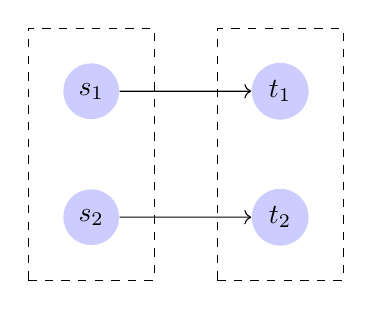
\begin{tikzpicture}
		[scale=.8,auto=left, every node/.style={circle,fill=blue!20}]
		\node (s1) at (1, 4) {$s_1$};
		\node (s2) at (1, 2)  {$s_2$};
		\node (t1) at (4, 4)  {$t_1$};
		\node (t2) at (4, 2) {$t_2$};

		\path (s1) edge [->](t1);
		\path (s2) edge [->](t2);

		\draw[dashed]  (0,1) -- (2, 1) -- (2, 5) -- (0, 5) -- (0, 1);
		\draw[dashed]  (3,1) -- (5, 1) -- (5, 5) -- (3, 5) -- (3, 1);

		\end{tikzpicture}
	\end{wrapfigure}
	
	Un grafo $G$ è costituito da:
	\begin{itemize}
		\item Un insieme di nodi $V$
		\item Un insieme di archi $E$
		\item $s: E \to V$ funzione sorgente
		\item $t: E \to V$ funzione destinazione
	\end{itemize}
	In altre parole, un grafo è un elemento di $$[E \mathrel{\mathop{\rightrightarrows}^{s}_{t}} V , \Set]$$.

	Un \emph{grafo con eqiuvalenza} $(G, \sim)$ è costituito da:
	\begin{itemize}
		\item Un grafo $G$
		\item Una relazione di quivalenza $\sim$ definita sui vertici
	\end{itemize}
	Ossia, un elemento di $[E \rightrightarrows V \to Q, \Set]$, tale che la freccia $q: V \to Q$ sia surgettiva (epi).

	Un E-Grafo $(G, \sim)$ è un grafo con equivalenza tale che
	\[
		\frac{s_G(e)\sim s_G(e')}{t_G(e) \sim t_G(e')}
	\]
\end{frame}

\begin{frame}[fragile]\frametitle{Pullback, Pushout, Equalizzatori}
	\begin{figure}[h]
		\begin{subfigure}{0.25\textwidth}
			\[\begin{tikzcd}[row sep = 20, column sep = 20]
				P' \arrow[dr, dashed, "v"] \arrow[drr, "{p_1'}", bend left=20] \arrow[ddr, "{p_2'}"swap, bend right=20] & & \\
 									& P \arrow[r, "{p_1}"] \arrow[d, "{p_2}"swap] 			& A \arrow[d, "f"] \\
									& B \arrow[r, "g"swap] 						& C
			\end{tikzcd}\]
			\caption{Pullback}
			\label{fig:pg}
		\end{subfigure}
		\qquad
		\begin{subfigure}{0.25\textwidth}
			\[\begin{tikzcd}[row sep = 20, column sep = 20]
				A \arrow[r, "f"] \arrow[d, "g"swap] 	& B \arrow[d, "{q_1}"] 	\arrow[ddr, "{q_1'}", bend left=20]	& \\
				C \arrow[r, "{q_2}"swap]  \arrow[drr, "{q_2'}"swap, bend right=20] & Q \arrow[dr, dashed, "u"] 	& \\
							& 				& Q'
			\end{tikzcd}\]
			\caption{Pushout}
			\label{po}
		\end{subfigure}
		\qquad
		\begin{subfigure}{0.25\textwidth}
			\[\begin{tikzcd}[row sep = 20, column sep = 20]
				E \arrow[r, "e"] & A \arrow[r, "f", shift left=1] \arrow[r,"g"swap, shift right = 1] & B \\
				E' \arrow[u, dashed, "h"] \arrow[ur, "{e'}"swap] &
			\end{tikzcd}\]
			\caption{Equalizzatore}
			\label{eq}
		\end{subfigure}
	\end{figure}

	In $\Set$:
	\begin{itemize}
		\item Pullback di $f$ e $g$: $ P = \{(x, y) \in A \times B \mid f(x) = g (y)\}$
		\item Pushout di $f$ e $g$:  $Q = (A \coprod B)/\sim$
		\item Equalizzatore di $f$ e $g$: $E=\{x \in A \mid f(x) = g(x)\}$
	\end{itemize}
\end{frame}

\begin{frame}[fragile]\frametitle{Adesività}


	\begin{wrapfigure}{ur}{0.4\textwidth}
                \[
                \begin{tikzcd}[row sep=11, column sep=11]
                        & {A'} && {B'} \\
                        {C'} && {D'} \\
                        & A && B \\
                        C && D
                        \arrow["{f'}", from=1-2, to=1-4]
                        \arrow["{m'}"', from=1-2, to=2-1]
                        \arrow["a"'{pos=0.7}, from=1-2, to=3-2]
                        \arrow["{n'}"', from=1-4, to=2-3]
                        \arrow["b", from=1-4, to=3-4]
                        \arrow["{g'}"{pos=0.7}, from=2-1, to=2-3, crossing over]
                        \arrow["c"', from=2-1, to=4-1]
                        \arrow["f"'{pos=0.3}, from=3-2, to=3-4]
                        \arrow["d"{pos=0.3}, from=2-3, to=4-3, crossing over]
                        \arrow["m", from=3-2, to=4-1]
                        \arrow["n", from=3-4, to=4-3]
                        \arrow["g"', from=4-1, to=4-3]
                    \end{tikzcd}
            \]
        \end{wrapfigure}
	Una categoria $\cat C$ è adesiva se:
	\begin{itemize}
		\item ha tutti i pushout di monomorfismi
		\item ha tutti i pullback
		\item i pushout di monomorfismi sono \emph{Van Kampen}
	\end{itemize}
\end{frame}

\begin{frame}[fragile]\frametitle{Approccio DPO su Categorie Adesive}
	Sia $\cat C$ una categoria adesiva.
	\begin{figure}[h]
		\begin{subfigure}{0.25\textwidth}
			\[\begin{tikzcd}[row sep = 20, column sep = 20] L & K \arrow[r, "r"] \arrow[l, "l"swap] & L \end{tikzcd}\]
		\label{fig:rule}
		\caption{Regola}
		\end{subfigure}
		\qquad
		\begin{subfigure}{0.25\textwidth}
			\[\begin{tikzcd}[row sep = 20, column sep = 20]
			L \arrow[d, "{m_L}"swap] & K\arrow[d, "{m_K}"] \arrow[r, "r"] \arrow[l, "l"swap] & R \arrow[d, "{m_R}"] \\
				G & D \arrow[l, "{l*}"] \arrow[r, "{r*}"swap] & H
		\end{tikzcd}\]
		\caption{Passo di derivazione}
		\label{fig:step}
		\end{subfigure}
	\end{figure}
	$l$ e $r$ sono due morfismi, possibilmente mono, di $\cat C$, 
	mentre i due quadrati sono pushout.


	\begin{figure}
		\includegraphics[width=0.4\linewidth]{imgs/fancyDPO}
	\end{figure}
\end{frame}

\end{document}
